% =====================================================================
%  Materials and Methods + Results, rewritten against the current pipeline
%  Batch: results/batches/paper_20260920_005408  (seeds 101, 202, 303)
%  Every number below is traceable to that batch's supplement export.
%  Figure sources are given in a comment above each \begin{figure}.
% =====================================================================

\section{Materials and Methods}
\label{sec:methods}

\subsection{Study population}
\label{sec:study_population}
This single-patient computational case study used clinical data collected at the National Center for Women and Children's Health, RSAB Harapan Kita, Jakarta, Indonesia, between December 2025 and June 2026. The protocol was approved by the Institutional Review Board of RSAB Harapan Kita (approval no.\ \textcolor{red}{[insert]}); written informed consent was obtained from the patient's legal guardian. Data were de-identified and the patient is referred to as P1.

Inclusion criteria were: (i) age above three months; (ii) VSD diagnosed by a pediatric cardiologist on clinical assessment and echocardiography; (iii) defect diameter $\ge 2$~mm; and (iv) scheduled transcatheter closure with anthropometric, echocardiographic and catheterization measurements sufficient to initialize and evaluate a patient-specific model. Exclusion criteria were: (i) missing or invalid core hemodynamic measurements; (ii) an additional severe cardiovascular abnormality expected to dominate the hemodynamics; and (iii) previous VSD closure or other corrective cardiac intervention. P1 was the first enrolled patient with a complete pre- and post-closure record. The design therefore supports a detailed evaluation of the workflow, not an estimate of performance across patients.

\subsection{Clinical data}
\label{sec:data}
Anthropometry, heart rate, defect anatomy, and invasive pressures and flows were taken from the catheterization protocol form and the echocardiography record (Table~\ref{tab:patient_data}). The effective defect diameter was the mean right-ventricular-side diameter reported in the procedure protocol ($D_{\mathrm{VSD}} = 3.665$~mm). Heart rate was taken per state and never shared between states (119~bpm pre-closure, 108~bpm post-closure).

Systemic mean arterial pressure was computed with the formula printed on the protocol form, $\overline{P} = (P_{\mathrm{sys}} + 2P_{\mathrm{dia}})/3$, applied to the right femoral artery (RFA) catheter readings, giving 71.33~mmHg pre-closure and 75.00~mmHg post-closure. The form additionally reports this formula applied to cuff readings (95.00 and 65.67~mmHg); those values are retained in the supplement as evaluation-only entries because cuff and catheter pressures disagree by more than 25\% in this record.

Post-closure measurements were acquired after the occluder had been deployed and the shunt was functionally closed. Two post-closure volume records exist and disagree: the patient's medical record (LVEDV/LVESV $=36.13/13.80$~mL) and rows 26--29 of the protocol form ($32.0/23.6$~mL). Following the study owner's confirmation that the thesis values originate from the medical record, the medical-record dataset is primary; the protocol-form dataset is declared as an alternative and both are evaluated (Section~\ref{sec:results_post}). No post-closure value entered calibration, parameter selection, priors or bounds at any point.

\begin{table}[ht]
\centering\small
\caption{Clinical record of P1. Pre-closure values marked \emph{fitted} entered the objective; all other entries were used for evaluation only. Post-closure values were withheld from calibration.}
\label{tab:patient_data}
\begin{tabular}{llrr}
\toprule
\textbf{Variable} & \textbf{Role} & \textbf{Pre-closure} & \textbf{Post-closure} \\
\midrule
Age (yr) / sex & input & 3.17 / \textcolor{red}{[insert]} & --- \\
Weight (kg) / height (cm) / BSA (m$^2$) & input & 13.4 / 95.0 / 0.588 & --- \\
Heart rate (bpm) & input & 119 & 108 \\
VSD type / diameter (mm) & input & perimembranous / 3.665 & occluded \\
\midrule
RFA pressure, sys/dia (mmHg) & fitted & 100 / 57 & 89 / 68 \\
Mean arterial pressure, RFA (mmHg) & fitted & 71.33 & 75.00 \\
PA pressure, sys/dia/mean (mmHg) & fitted & 20 / 10 / 15 & 17 / 9 / 13 \\
RA mean pressure (mmHg) & fitted & 5 & 5 \\
Systemic flow $Q_s$ (L/min) & fitted & 3.423 & 2.54$^{\mathrm{a}}$ \\
$Q_p/Q_s$ (--) & fitted & 1.194 & 0.90$^{\mathrm{a}}$ \\
Shunt flow (L/min) & fitted$^{\mathrm{b}}$ & 0.664 & --- \\
\midrule
Pulmonary flow $Q_p$ (L/min) & evaluation & 4.087 & --- \\
SVR (WU) & evaluation & 19.38 & 27.56$^{\mathrm{a}}$ \\
LV / RV systolic pressure (mmHg) & evaluation & 94 / 25 & --- \\
DAo pressure, sys/dia (mmHg) & evaluation & 91 / 57 & 104.3 / 71.7 \\
Cuff pressure, sys/dia (mmHg) & evaluation & 119 / 83 & 86.7 / 55.3 \\
LVEDV / LVESV (mL) & evaluation & --- & 36.13 / 13.80$^{\mathrm{a}}$ \\
RVEDV / RVESV (mL) & evaluation & --- & 30.5 / 12.0$^{\mathrm{a}}$ \\
LVEF / RVEF (--) & evaluation & --- & 0.618 / 0.607$^{\mathrm{a}}$ \\
\bottomrule
\end{tabular}
\par\vspace{2pt}
\footnotesize{$^{\mathrm{a}}$Medical-record dataset (primary). The protocol form reports LVEDV/LVESV $=32.0/23.6$~mL (LVEF 0.263) for the same state; both are evaluated in Section~\ref{sec:results_post}. $^{\mathrm{b}}$Included in the objective but excluded from the governed error metric (Section~\ref{sec:statistics}).}
\end{table}

% FIGURE SOURCE: docs/manuscript/figures/Flowchart.png  (existing workflow diagram)
\begin{figure}[ht]
\centering
\includegraphics[width=0.78\linewidth]{figures/Flowchart.png}
\caption{Patient-specific modeling workflow. The clinical record scales and seeds the model, global sensitivity analysis selects the parameters to be fitted, staged multi-start optimization calibrates the pre-closure state, the calibrated set is audited for practical identifiability, and the same set is applied unchanged with the shunt closed to predict the withheld post-closure state.}
\label{fig:workflow}
\end{figure}

\subsection{Model}
\label{sec:model}

\subsubsection{Structure}
The circulation is a closed-loop lumped-parameter network adapted from the intracardiac-shunt architecture of Ferrero et al.~\cite{Ferrero2026Shunts} (Figure~\ref{fig:schematic}): four time-varying elastance chambers, a systemic circuit (arterial, capillary and venous compartments), a pulmonary circuit (arterial compartment, parallel oxygenated and non-oxygenated capillary branches, venous compartment), four valves, and an interventricular shunt. Vascular compartments use resistance--compliance--inertance elements~\cite{Shi2011}. Equations~(\ref{eq:state})--(\ref{eq:elastance}) are standard and are reproduced only where needed to define symbols; the two relations modified in this work are identified explicitly in Section~\ref{sec:valves}.

The state vector has 14 entries,
\begin{equation}
\mathbf{X} = \left[ V_{\mathrm{RA}}, V_{\mathrm{RV}}, V_{\mathrm{LA}}, V_{\mathrm{LV}}, V_{\mathrm{SAR}}, Q_{\mathrm{SAR}}, V_{\mathrm{SC}}, V_{\mathrm{SVEN}}, Q_{\mathrm{SVEN}}, V_{\mathrm{PAR}}, Q_{\mathrm{PAR}}, P_{\mathrm{PC}}, V_{\mathrm{PVEN}}, Q_{\mathrm{PVEN}} \right]^{\top},
\label{eq:state}
\end{equation}
with volumes $V$ (mL), flows $Q$ (mL/s) and the pulmonary capillary pressure $P_{\mathrm{PC}}$ (mmHg). Chamber volumes obey
\begin{equation}
\begin{aligned}
\dot{V}_{\mathrm{RA}} &= Q_{\mathrm{SVEN}} - Q_{\mathrm{TV}}, &
\dot{V}_{\mathrm{RV}} &= Q_{\mathrm{TV}} + Q_{\mathrm{VSD}} - Q_{\mathrm{PV}}, \\
\dot{V}_{\mathrm{LA}} &= Q_{\mathrm{PVEN}} - Q_{\mathrm{MV}}, &
\dot{V}_{\mathrm{LV}} &= Q_{\mathrm{MV}} - Q_{\mathrm{AV}} - Q_{\mathrm{VSD}},
\end{aligned}
\label{eq:chambers}
\end{equation}
and the compartment mass and momentum balances are given in Appendix~\ref{app:circuit}. Nominal adult reference values are listed in Appendix~\ref{app:nominal_parameters}.

% FIGURE SOURCE: docs/manuscript/figures/model_schematic.pdf  (circuitikz; source model_schematic.tex)
\begin{figure}[ht]
\centering
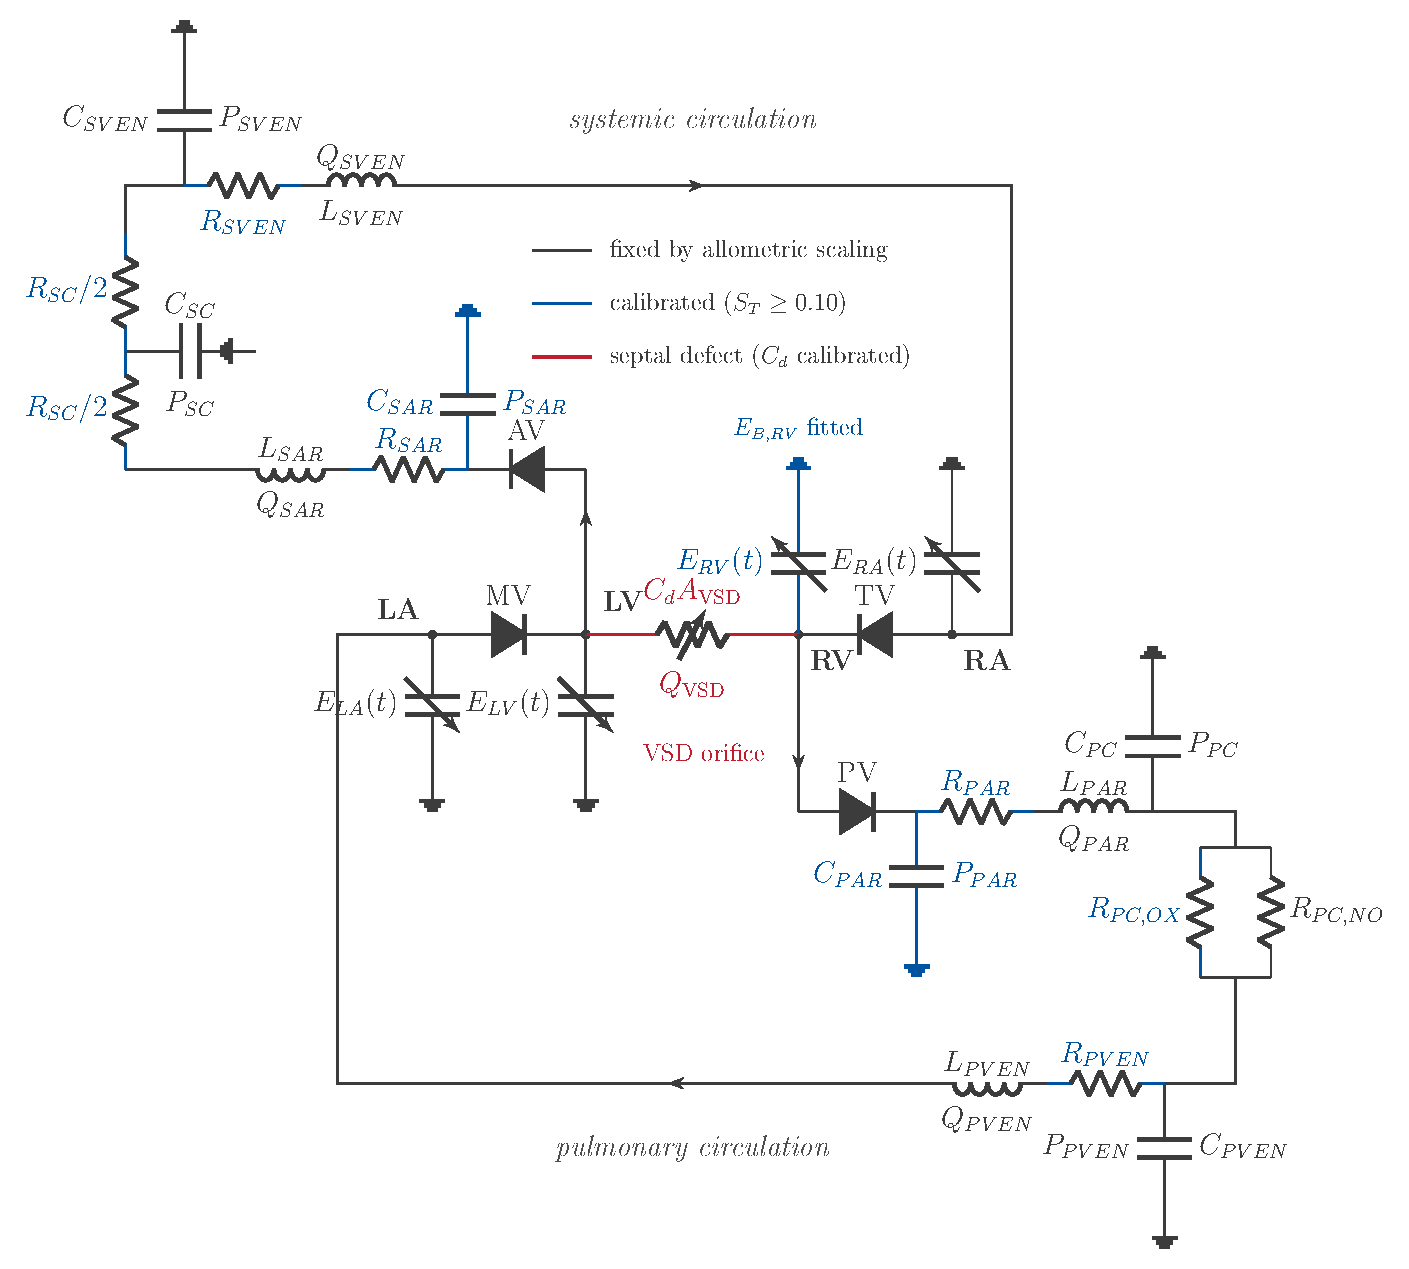
\includegraphics[width=\linewidth]{figures/model_schematic.pdf}
\caption{Electrical analogue of the closed-loop model. Chambers are time-varying elastances, valves are smooth diodes, and the interventricular defect is an orifice between the ventricles. Blue elements are the seven parameters selected by the sensitivity screen and fitted during calibration (Section~\ref{sec:gsa}); grey elements are held at their allometrically scaled values.}
\label{fig:schematic}
\end{figure}

\subsubsection{Cardiac chambers}
Chamber pressure follows the time-varying elastance concept~\cite{Suga1974,Walley2016},
\begin{equation}
P_{ch}(t) = E_{ch}(t)\left(V_{ch}(t) - V_{0,ch}\right), \qquad
E_{ch}(t) = E_{\mathrm{B},ch} + E_{\mathrm{A},ch}\, e_{ch}(t),
\label{eq:elastance}
\end{equation}
with unstressed volume $V_{0,ch}$, passive elastance $E_{\mathrm{B},ch}$, active amplitude $E_{\mathrm{A},ch}$ and normalized activation $e_{ch}(t)\in[0,1]$. Ventricular activation over the cardiac phase $\phi = \mathrm{mod}(t, T_{\mathrm{HB}})$, $T_{\mathrm{HB}} = 60/\mathrm{HR}$, is the piecewise cosine of Colebank et al.~\cite{Colebank2026} and Ferrero et al.~\cite{Ferrero2026Shunts},
\begin{equation}
e_v(\phi) =
\begin{cases}
\tfrac{1}{2}\left[1-\cos\left(\pi\phi/T_{vc}\right)\right], & 0 \le \phi \le T_{vc},\\[3pt]
\tfrac{1}{2}\left[1+\cos\left(\pi(\phi-T_{vc})/T_{vr}\right)\right], & T_{vc} < \phi \le T_{vc}+T_{vr},\\[3pt]
0, & \text{otherwise},
\end{cases}
\label{eq:activation}
\end{equation}
where $T_{vc}$ and $T_{vr}$ are the contraction and relaxation durations, specified as fractions of $T_{\mathrm{HB}}$ so that the timing rescales with heart rate. Atrial activation uses the same form evaluated at $\tau = \mathrm{mod}(\phi - t_{ac}, T_{\mathrm{HB}})$, with $t_{ac}$ the onset of atrial contraction in late diastole.

\subsubsection{Valves and interventricular shunt}
\label{sec:valves}
Ideal diodes introduce discontinuities that degrade stiff integration. Each valve is therefore a smooth gate between an open and a closed resistance, the continuous-switch approach used in closed-loop lumped-parameter models~\cite{Shi2011}; the specific hyperbolic-tangent form below is the implementation adopted in this work,
\begin{equation}
g = \tfrac{1}{2} + \tfrac{1}{2}\tanh\!\left(\frac{\Delta P}{\varepsilon_{\mathrm{v}}}\right), \qquad
Q_{\mathrm{valve}} = \Delta P\left(\frac{g}{R_{\mathrm{open}}} + \frac{1-g}{R_{\mathrm{closed}}}\right),
\label{eq:valve}
\end{equation}
with transvalvular gradient $\Delta P$, $\varepsilon_{\mathrm{v}} = 0.5$~mmHg, $R_{\mathrm{open}} = 4.0\times10^{-3}$ and $R_{\mathrm{closed}} = 9.42\times10^{4}$~mmHg\,s/mL.

Shunt flow uses the Gorlin orifice relation~\cite{Gorlin1951}. The square-root law is unmodified; the sign-preserving factor that makes it differentiable through zero gradient is introduced here,
\begin{equation}
Q_{\mathrm{VSD}} = C_d\, A_{\mathrm{VSD}} \sqrt{\frac{2\,\gamma\,\lvert\Delta P_{\mathrm{v}}\rvert}{\rho}}\;
\underbrace{\frac{\Delta P_{\mathrm{v}}}{\sqrt{\Delta P_{\mathrm{v}}^{2} + \varepsilon_{\mathrm{s}}^{2}}}}_{\text{smoothing (this work)}},
\qquad A_{\mathrm{VSD}} = \pi\left(\frac{D_{\mathrm{VSD}}}{2}\right)^{2},
\label{eq:orifice}
\end{equation}
where $\Delta P_{\mathrm{v}} = P_{\mathrm{LV}} - P_{\mathrm{RV}}$ (positive left-to-right), $\rho = 1060$~kg/m$^3$, $\gamma = 133.322$~Pa/mmHg and $\varepsilon_{\mathrm{s}} = 0.1$~mmHg. The discharge coefficient $C_d$ lumps defect shape and flow contraction and is the only shunt parameter calibrated. Closure is imposed by setting $A_{\mathrm{VSD}} = 0$ and $R_{\mathrm{VSD}} = 10^{6}$~mmHg\,s/mL; $Q_{\mathrm{VSD}} \approx 0$ was verified numerically in every post-closure simulation.

\subsubsection{Pediatric scaling}
Adult reference parameters were scaled by the weight-based allometric law of Zhang et al.~\cite{zhang2019multiscale},
\begin{equation}
\theta_i = \theta_{i,\mathrm{ref}} \left(\frac{W_{\mathrm{p}}}{W_{\mathrm{ref}}}\right)^{\alpha_i},
\label{eq:scaling}
\end{equation}
with $W_{\mathrm{ref}} = 70$~kg, $W_{\mathrm{p}} = 13.4$~kg and the class exponents of Table~\ref{tab:exponents}. Zhang et al.\ report no exponent for inertance; $\alpha = -1$ was adopted from the mechanical-similarity argument of Lundquist et al.~\cite{Lundquist2025} and is the only exponent not taken from~\cite{zhang2019multiscale}. The age-dependent maturation correction of systemic and pulmonary resistance described by Colebank et al.~\cite{Colebank2026} is implemented; at the age of P1 (1158 days) both correction factors equal 1.000, so it has no effect here. No alternative scaling law was applied.

\begin{table}[ht]
\centering\small
\caption{Weight-based allometric exponents used in Eq.~(\ref{eq:scaling}).}
\label{tab:exponents}
\begin{tabular}{llc}
\toprule
\textbf{Class} & \textbf{Parameters} & $\alpha_i$ \\
\midrule
Heart rate & HR & $-0.30$ \\
Left-heart elastance & $E_{\mathrm{A/B,LV}}$, $E_{\mathrm{A/B,LA}}$ & $-0.50$ \\
Right-heart elastance & $E_{\mathrm{A/B,RV}}$, $E_{\mathrm{A/B,RA}}$ & $-0.75$ \\
Systemic resistance & $R_{\mathrm{SAR}}$, $R_{\mathrm{SC}}$, $R_{\mathrm{SVEN}}$ & $-0.475$ \\
Pulmonary resistance & $R_{\mathrm{PAR}}$, $R_{\mathrm{PCOX}}$, $R_{\mathrm{PCNO}}$, $R_{\mathrm{PVEN}}$ & $-0.70$ \\
Compliance & all vascular $C$ & $+1.00$ \\
Unstressed volume & all $V_0$ & $+0.80$ \\
Inertance & all $L$ & $-1.00$\,$^{\mathrm{a}}$ \\
Valve open resistance & $R_{\mathrm{open}}$ & $-0.50$ \\
\bottomrule
\end{tabular}
\par\vspace{2pt}
\footnotesize{$^{\mathrm{a}}$From Lundquist et al.~\cite{Lundquist2025}; all other exponents from Zhang et al.~\cite{zhang2019multiscale}.}
\end{table}

\subsubsection{Initialization and clinical seeding}
Total blood volume was $\mathrm{BV} = W_{\mathrm{p}}\,\nu$ with $\nu = 70$~mL/kg above one year of age (82~mL/kg below)~\textcolor{red}{[cite source of 70/82 mL/kg]}, giving 938~mL. Initial volumes were $V_i(0) = V_{0,i} + P_{\mathrm{nom},i} C_i$ for vascular compartments and $V_{ch}(0) = V_{0,ch} + P_{\mathrm{ED},ch}/E_{\mathrm{B},ch}$ for chambers, with nominal pressures from the pre-closure record. The systemic venous unstressed volume closes the volume budget,
\begin{equation}
V_{0,\mathrm{SVEN}} = \mathrm{BV} - \sum_{i \neq \mathrm{SVEN}} V_i(0) - P_{\mathrm{nom,SVEN}}\,C_{\mathrm{SVEN}},
\label{eq:sven}
\end{equation}
bounded to $[\max(0.01\,\mathrm{BV},\,1~\mathrm{mL}),\ 0.85\,\mathrm{BV}]$. Equation~(\ref{eq:sven}) is a bookkeeping constraint specific to this implementation.

Before calibration, the measured aggregate resistances were distributed over the compartments in proportion to their scaled values, $R_i \leftarrow R_i\,\mathrm{SVR}/(R_{\mathrm{SAR}}+R_{\mathrm{SC}}+R_{\mathrm{SVEN}})$ systemically and analogously for the pulmonary circuit. Arterial compliances were anchored to stroke volume over pulse pressure, $C_{\mathrm{SAR}} = \mathrm{SV}_{\mathrm{s}}/\mathrm{PP}_{\mathrm{s}}$ and $C_{\mathrm{PAR}} = \mathrm{SV}_{\mathrm{p}}/\mathrm{PP}_{\mathrm{p}}$~\cite{Colebank2026}. The discharge coefficient was seeded by inverting Eq.~(\ref{eq:orifice}) with the measured shunt flow, giving $C_d^{(0)} = 0.356$.

\subsubsection{Numerical solution}
The system was integrated with \texttt{ode15s}~\cite{Shampine1997} in MATLAB R2025a (relative tolerance $10^{-5}$, absolute $10^{-6}$, maximum step $T_{\mathrm{HB}}/50$). Cycles were advanced until peak pressures and volumes changed by less than 0.1~mmHg and 0.1~mL between consecutive cycles (maximum 80 cycles); outputs were computed from the final two cycles. Periodic steady state was reached in every simulation reported here.

\subsection{Parameter screening and calibration}
\label{sec:calibration}

\subsubsection{Global sensitivity analysis}
\label{sec:gsa}
Variance-based global sensitivity analysis~\cite{Sobol2001,Saltelli2010}, following recommendations for cardiovascular models~\cite{Eck2016}, ranked the parameters by their influence on the model outputs. Sparse polynomial chaos expansions~\cite{Blatman2011} were fitted in UQLab~\cite{Marelli2014} (LARS, degree 1--3, hyperbolic truncation $q = 0.75$) to one shared Halton design of $N = 128$ points over $d = 21$ independent uniform inputs. Input ranges were $[0.4,\,2.5]\,x_0$ for resistances, $[0.5,\,2.0]\,x_0$ for compliances and elastances, $[0.6,\,1.7]\,x_0$ for unstressed volumes and $[0.8,\,1.2]\,x_0$ for $C_d$. Total-order Sobol' indices were obtained analytically from the expansion coefficients~\cite{Sudret2008},
\begin{equation}
S_{T_i} = 1 - \frac{\mathrm{Var}\!\left(\mathbb{E}\left[Y \mid \mathbf{X}_{\sim i}\right]\right)}{\mathrm{Var}(Y)},
\label{eq:sobol}
\end{equation}
for 25 outputs. A candidate parameter was retained for calibration if $S_{T_i} \ge 0.10$ for at least one governed target; coupled resistance groups inherit the largest index of their members. The screen was repeated at the calibrated operating point. A 128-point design supports ranking rather than precise index values, and the indices are reported as a screening result.

\subsubsection{Objective function and staged multi-start optimization}
Calibration minimized
\begin{equation}
J(\mathbf{x}) = \sum_{k \in \mathcal{H}} w_k\left(\frac{\varepsilon_k}{\tau_{\mathcal{H}}}\right)^{2}
+ \sum_{k \in \mathcal{S}} w_k\left(\frac{\varepsilon_k}{\tau_{\mathcal{S}}}\right)^{2}
+ \lambda_{\mathrm{p}}\sum_{j} c_j \ln^{2}\!\left(\frac{x_j}{x_j^{\mathrm{s}}}\right) + J_{\mathrm{b}},
\qquad \varepsilon_k = \frac{y_k(\mathbf{x}) - y_k^{\mathrm{clin}}}{y_k^{\mathrm{clin}}},
\label{eq:objective}
\end{equation}
where $\mathcal{H}$ and $\mathcal{S}$ are the hard and soft target sets (Section~\ref{sec:statistics}) with tolerances $\tau_{\mathcal{H}} = 0.05$ and $\tau_{\mathcal{S}} = 0.10$ and weights $w_k$. The third term penalizes drift from the scaled value $x_j^{\mathrm{s}}$ in proportion to prior confidence $c_j$ ($\lambda_{\mathrm{p}} = 0.5$), and $J_{\mathrm{b}}$ penalizes parameters resting on their bounds. Mean right atrial pressure, mean systemic pressure and cardiac output enter as one coupled systemic term so that a single systemic load is not counted three times. Equation~(\ref{eq:objective}) is specific to this work.

Only the parameters retained by the screen were fitted; the screen is binding, and no stage may introduce a parameter outside it. For each starting point, a staged sequence of bound-constrained subproblems was solved with \texttt{fmincon} (interior-point; sequential quadratic programming in the final stage): vascular parameters and $C_d$ (stage A), chamber parameters (stage B), the five highest-ranked retained parameters jointly (stage C), then three refinements targeting the systemic outputs, parameter plausibility and the acceptance gate (stages D--F). A refinement was kept only if it increased neither the governed error nor the number of gate failures. Six starting points were used: the clinically seeded vector and five scrambled Sobol' points inside the bounds. The accepted candidate was chosen lexicographically: fewest hard-target failures, then fewest gate failures, then lowest governed RMSE.

The complete pipeline was executed three times with the multi-start seeds 101, 202 and 303, fixed in advance, with clinical inputs and all other settings held constant. The seed enters only through the scrambling of starting points 2--6; starting point 1 is deterministic. All three runs are reported.

\begin{table}[ht]
\centering\small
\caption{The seven parameters retained by the sensitivity screen: allometrically scaled value, clinically seeded start, bounds, and the calibrated value (identical in all three runs). Resistance scales are dimensionless multipliers of the scaled compartment values.}
\label{tab:bounds}
\begin{tabular}{llrrrrrr}
\toprule
\textbf{Parameter} & \textbf{Unit} & \textbf{Scaled} & \textbf{Seed} & \textbf{lb} & \textbf{ub} & \textbf{Calibrated} & \textbf{Ratio} \\
\midrule
$R_{\mathrm{sys}}$ scale ($R_{\mathrm{SAR}}$, $R_{\mathrm{SC}}$) & -- & 1.0000 & 1.0000 & 0.2500 & 2.8000 & 0.5686 & 0.57 \\
$R_{\mathrm{SVEN}}$ & mmHg\,s/mL & 0.1097 & 0.1097 & 0.0439 & 0.3070 & 0.1655 & 1.51 \\
$R_{\mathrm{pul}}$ scale ($R_{\mathrm{PAR}}$, $R_{\mathrm{PCOX}}$, $R_{\mathrm{PVEN}}$) & -- & 1.0000 & 1.0000 & 0.4500 & 2.8000 & 0.4500$^{\ast}$ & 0.45 \\
$C_{\mathrm{SAR}}$ & mL/mmHg & 0.2546 & 0.6689 & 0.2419 & 0.9031 & 0.5703 & 2.24 \\
$C_{\mathrm{PAR}}$ & mL/mmHg & 0.9571 & 3.4345 & 0.9056 & 4.9800 & 1.0170 & 1.06 \\
$E_{\mathrm{B,RV}}$ & mmHg/mL & 0.1451 & 0.1451 & 0.0798 & 0.3773 & 0.0799$^{\ast}$ & 0.55 \\
$C_d$ & -- & 0.7000 & 0.3561 & 0.2849 & 0.7350 & 0.3697 & 0.53 \\
\bottomrule
\end{tabular}
\par\vspace{2pt}
\footnotesize{$^{\ast}$Converged onto the lower bound (within $10^{-4}$ of it).}
\end{table}

\subsubsection{Post-closure prediction}
\label{sec:post_methods}
The post-closure state is a prediction, not a fit. The calibrated pre-closure parameter set was applied unchanged with the defect closed and the heart rate set to its measured post-closure value (108~bpm); no parameter was refitted and no post-closure measurement influenced calibration. Differences from the withheld measurements are therefore attributable to the model together with its pre-closure parameters. A post-closure calibration, which would test whether the post-closure state is representable at all, was not performed here and is identified as future work.

\subsubsection{Practical identifiability}
\label{sec:identifiability}
Practical identifiability was assessed at the calibrated operating point from the scaled sensitivity matrix~\cite{Pope2009,Olufsen2013}
\begin{equation}
S_{ij} = \frac{\partial y_i}{\partial \theta_j}\,\frac{\theta_j}{\sigma_i},
\label{eq:sensitivity}
\end{equation}
with $\sigma_i$ the declared measurement uncertainty of target $i$. Parameters with small column norms are weakly constrained; pairs with $\lvert\rho\rvert \ge 0.9$ between columns were flagged as collinear. The condition number $\mathrm{cond}(S)$ was evaluated for every subset of size $k \le p$ and the best-conditioned subset at each size reported as a candidate reduced set~\cite{vanOsta2020}. Subsets were scored by linear algebra alone, without re-simulation or recalibration.

\subsection{Statistical analysis}
\label{sec:statistics}
Each target $k$ was summarized by the signed relative error $\varepsilon_k$ of Eq.~(\ref{eq:objective}) and aggregated as the governed root-mean-square error over the $K$ governed targets,
\begin{equation}
\mathrm{RMSE} = \sqrt{\frac{1}{K}\sum_{k=1}^{K}\varepsilon_k^{2}},
\label{eq:rmse}
\end{equation}
evaluated for the scaled baseline and after calibration.

Targets were assigned one of four tiers, fixed before the runs:
\begin{itemize}[leftmargin=1.5em]
\item \textbf{Hard (H)} --- directly measured, low-uncertainty quantities that must be matched: mean right atrial, mean pulmonary arterial and mean systemic arterial pressure, systemic flow and $Q_p/Q_s$ (5 targets).
\item \textbf{Soft (S)} --- measured but method-sensitive extremes, matched with a wider tolerance: systolic and diastolic pulmonary and systemic pressure (4 targets).
\item \textbf{Held out of the governed metric} --- used in the objective but excluded from the reported RMSE because it is a derived difference of two fitted flows: shunt flow.
\item \textbf{Derived validation} --- never used in the objective and reported for validation only: SVR, and every post-closure quantity.
\end{itemize}
The 5 hard and 4 soft targets form the $K = 9$ governed targets. A target passes the acceptance gate when $\lvert\varepsilon_k\rvert \le 10\%$. A run is \emph{accepted} when all governed targets pass and all parameters satisfy the plausibility bounds, \emph{physiological but poor fit} when the parameters are plausible but the gate is not met, and \emph{not accepted} otherwise.

Goodness of fit was also reported as $\chi^2 = \sum_k z_k^2$ with $z_k = (y_k^{\mathrm{model}} - y_k^{\mathrm{clin}})/\sigma_k$, where $\sigma_k$ is the declared uncertainty of target $k$ (5\% for catheter mean pressures and $Q_p/Q_s$, 10\% for pressure extremes, 15\% for flows, 20\% for derived quantities). Both $\chi^2/N$ per observation and the reduced $\chi^2$ over the degrees of freedom $N - p$ are given, interpreted descriptively.

Because one patient was studied, no between-patient statistics were computed. Results are reported per run; agreement between runs measures the numerical reproducibility of the pipeline, not variability across patients.

\subsection{Measurement-noise simulation}
\label{sec:noise}
\textcolor{red}{[PLACEHOLDER --- to be written after the noise runs. Scope agreed: the three fixed-seed repeats test only the stochastic component of the multi-start search, which is deterministic once the seeded start wins (Section~\ref{sec:results_multistart}). A separate Monte Carlo experiment will perturb each clinical target within its declared measurement uncertainty, recalibrate, and report the resulting distribution of calibrated parameters and predicted post-closure outputs. This subsection will state the number of noise replicates, the perturbation model, and the summary statistics reported.]}

% =====================================================================
\section{Results}
\label{sec:results}

\subsection{Parameter screening}
\label{sec:results_gsa}
The screen retained 7 of the 14 candidate parameters (Table~\ref{tab:bounds}; Figure~\ref{fig:gsa_screen}). Ranked by the largest total-order index across the governed targets, these were the systemic resistance scale ($S_T = 0.70$), the discharge coefficient $C_d$ (0.51), the passive right-ventricular elastance $E_{\mathrm{B,RV}}$ (0.48), the pulmonary resistance scale (0.40), the pulmonary arterial compliance $C_{\mathrm{PAR}}$ (0.39), the systemic arterial compliance $C_{\mathrm{SAR}}$ (0.12) and the systemic venous resistance $R_{\mathrm{SVEN}}$ (0.10). Seven candidates fell below the threshold for every governed target: $E_{\mathrm{A,RV}}$ (0.080), $E_{\mathrm{B,LV}}$ (0.073), $E_{\mathrm{A,LV}}$ (0.031), $E_{\mathrm{A,RA}}$ (0.006), $E_{\mathrm{A,LA}}$ (0.005), $V_{0,\mathrm{RV}}$ (0.004) and $V_{0,\mathrm{LV}}$ (0.001).

Individual outputs were governed by few parameters. Mean systemic pressure was dominated by the systemic capillary resistance $R_{\mathrm{SC}}$ ($S_T = 0.58$), which also led cardiac output (0.33); $Q_p/Q_s$ by $C_d$ (0.51) with $R_{\mathrm{SC}}$ (0.41); mean right atrial pressure by $E_{\mathrm{B,RV}}$ (0.48); and mean pulmonary pressure by the pulmonary capillary resistance $R_{\mathrm{PCOX}}$ (0.30) with $C_{\mathrm{PAR}}$ (0.20). The ranking was unchanged when the screen was repeated at the calibrated operating point.

The parameters excluded by the screen nonetheless controlled the unmeasured chamber outputs: $E_{\mathrm{A,LV}}$ dominated LVESV ($S_T = 0.59$) and LVEF (0.63), and $E_{\mathrm{A,RV}}$ dominated RVESV (0.71) and RVEF (0.76). Because no chamber volume was measured before closure, these parameters were not constrained by any governed target. Surrogate accuracy was adequate for screening, with modified leave-one-out errors of 0.043--0.155 across the 25 outputs.

% FIGURE SOURCE: results/batches/paper_20260920_005408/figures/F01_gsa_tornado_screening.pdf
\begin{figure}[ht]
\centering
\includegraphics[width=0.85\linewidth]{figures/F01_gsa_tornado_screening.pdf}
\caption{Total-order Sobol' indices at the scaled baseline, by parameter and output. The dashed line marks the retention threshold $S_T = 0.10$. Parameters above the threshold for at least one governed target were calibrated; the rest were held fixed.}
\label{fig:gsa_screen}
\end{figure}

\subsection{Pre-closure calibration}
\label{sec:results_pre}
Calibration reduced the governed RMSE from 0.2738 at the scaled baseline to 0.1047, an improvement of 61.7\%, and 7 of the 9 governed targets fell inside the 10\% gate (Table~\ref{tab:pre_targets}, Figure~\ref{fig:calibration}). All five hard targets passed, with absolute errors of 4.6\% (mean RAP), 5.5\% (mean PAP), 2.5\% (mean SAP), 8.0\% (systemic flow) and 3.1\% ($Q_p/Q_s$). Two soft targets failed: pulmonary systolic pressure was over-predicted by 25.5\% (25.1 against 20~mmHg) and systemic systolic pressure under-predicted by 11.9\% (88.1 against 100~mmHg). Shunt flow, which is used in the objective but held out of the governed metric, was under-predicted by 25.3\% (0.496 against 0.664~L/min). SVR, used for validation only, agreed to 5.4\%. All three runs returned the identical calibrated parameter set and therefore identical values in Table~\ref{tab:pre_targets}; the reason is given in Section~\ref{sec:results_multistart}.

Every run was classified \emph{physiological but poor fit}: the parameters remained inside their plausibility bounds but the gate was not met. With $\chi^2 = 31.30$ over 9 observations, $\chi^2/N = 3.48$, and with 7 fitted parameters the reduced $\chi^2$ is 15.65 on 2 degrees of freedom. The largest standardized residual was pulmonary systolic pressure ($z = 5.10$). The fit is therefore worse than the declared measurement uncertainties allow, and is reported as such.

Two of the seven calibrated parameters converged onto their lower bounds (the pulmonary resistance scale and $E_{\mathrm{B,RV}}$, Table~\ref{tab:bounds}), indicating that the objective would have preferred values outside the physiologically admissible range. Of the parameters that moved freely, the systemic resistance scale fell to 0.57 of its scaled value, $C_{\mathrm{SAR}}$ rose to 2.24 times, $R_{\mathrm{SVEN}}$ to 1.51 times, $C_{\mathrm{PAR}}$ was essentially unchanged (1.06), and $C_d$ settled at 0.370, close to its clinically seeded value of 0.356 and well below the adult reference of 0.70.

\begin{table}[ht]
\centering\small
\setlength{\tabcolsep}{4pt}
\caption{Pre-closure targets: measurement, scaled baseline and calibrated model. Tier as defined in Section~\ref{sec:statistics}: H = hard, S = soft, HO = used in the objective but held out of the governed metric, DV = derived validation, not used in the objective. Values are identical in all three runs.}
\label{tab:pre_targets}
\begin{tabular}{llrrrrrc}
\toprule
\textbf{Target} & \textbf{Tier} & \textbf{Measured} & \textbf{Baseline} & $\varepsilon$ (\%) & \textbf{Calibrated} & $\varepsilon$ (\%) & \textbf{Gate} \\
\midrule
Mean RA pressure (mmHg) & H & 5.00 & 5.05 & $+1.1$ & 5.23 & $+4.6$ & pass \\
Mean PA pressure (mmHg) & H & 15.00 & 19.05 & $+27.0$ & 15.82 & $+5.5$ & pass \\
Mean systemic pressure (mmHg) & H & 71.33 & 77.04 & $+8.0$ & 69.56 & $-2.5$ & pass \\
Systemic flow $Q_s$ (L/min) & H & 3.423 & 2.188 & $-36.1$ & 3.149 & $-8.0$ & pass \\
$Q_p/Q_s$ (--) & H & 1.194 & 1.201 & $+0.6$ & 1.157 & $-3.1$ & pass \\
PA diastolic pressure (mmHg) & S & 10.00 & 16.50 & $+65.0$ & 9.70 & $-3.0$ & pass \\
PA systolic pressure (mmHg) & S & 20.00 & 21.41 & $+7.1$ & 25.10 & $+25.5$ & \textbf{fail} \\
Systemic diastolic pressure (mmHg) & S & 57.00 & 65.75 & $+15.4$ & 52.75 & $-7.5$ & pass \\
Systemic systolic pressure (mmHg) & S & 100.00 & 88.19 & $-11.8$ & 88.09 & $-11.9$ & \textbf{fail} \\
\midrule
Shunt flow (L/min) & HO & 0.664 & 0.441 & $-33.7$ & 0.496 & $-25.3$ & --- \\
SVR (WU) & DV & 19.38 & 32.90 & $+69.8$ & 20.43 & $+5.4$ & --- \\
\midrule
Governed RMSE & & --- & 0.2738 & & 0.1047 & & \\
Governed gate & & --- & --- & & 7/9 & & \\
$\chi^2/N$ ($N=9$) & & --- & --- & & 3.48 & & \\
Status & & --- & --- & & \multicolumn{3}{l}{Physiological but poor fit} \\
\bottomrule
\end{tabular}
\end{table}

% FIGURE SOURCE: results/batches/paper_20260920_005408/figures/F03_calibration_before_after.pdf
\begin{figure}[ht]
\centering
\includegraphics[width=0.85\linewidth]{figures/F03_calibration_before_after.pdf}
\caption{Relative error of each governed target at the scaled baseline and after calibration, for all three runs. The shaded band is the $\pm10\%$ acceptance gate.}
\label{fig:calibration}
\end{figure}

\subsection{Simulated hemodynamics}
\label{sec:results_hemo}
The calibrated model produced physiological waveforms and a purely left-to-right shunt through the cardiac cycle (Figure~\ref{fig:pvloops}). Simulated pulmonary flow was 3.64~L/min against a systemic flow of 3.15~L/min, and mean left atrial pressure was 7.8~mmHg. The shunt carried 13.6\% of pulmonary flow.

Chamber volumes, for which no pre-closure measurement exists, were LVEDV 39.8~mL, LVESV 9.8~mL and LVEF 0.75, and RVEDV 43.3~mL, RVESV 14.9~mL and RVEF 0.65. All fall inside the pediatric plausibility ranges used in the audit, but none is constrained by data; the sensitivity screen showed that the parameters controlling them were excluded precisely because no measurement governs them (Section~\ref{sec:results_gsa}).

% FIGURE SOURCE: results/batches/paper_20260920_005408/figures/F07_pressure_volume_loops.pdf
\begin{figure}[ht]
\centering
\includegraphics[width=0.85\linewidth]{figures/F07_pressure_volume_loops.pdf}
\caption{Left and right ventricular pressure--volume loops of the calibrated pre-closure state and of the post-closure prediction. Pressure waveforms and the shunt-flow trace are given in the supplementary material.}
\label{fig:pvloops}
\end{figure}

\subsection{Multi-start behaviour and run-to-run reproducibility}
\label{sec:results_multistart}
The three runs returned the same accepted parameter set, so the pipeline is exactly reproducible under the seeds tested. The reason is visible in the multi-start record (Table~\ref{tab:multistart}): the clinically seeded starting point is deterministic and is not affected by the seed, it was the only start with no hard-target failure and the lowest governed error in runs 101 and 202, and it won the lexicographic selection in all three runs. The seed changes only the five scrambled starting points.

Variability therefore exists between starting points rather than between runs. Across the 18 starts, the governed RMSE ranged from 0.0909 to 0.1509. One scrambled start in run 303 reached 0.0909, below the accepted value of 0.1047, but failed one hard target and was rejected by the selection rule. This is the intended behaviour of the rule, and it means the reported result is not the lowest error attained, but the lowest error attained without a hard-target failure.

Because the accepted candidate does not vary, the three repeats do not quantify uncertainty. The measurement-noise experiment of Section~\ref{sec:noise} is the analysis intended for that purpose.

\begin{table}[ht]
\centering\small
\caption{Governed RMSE of the six starting points in each run, with the number of hard-target failures and gate failures in parentheses. The selected start is in bold.}
\label{tab:multistart}
\begin{tabular}{lccc}
\toprule
\textbf{Start} & \textbf{Run 101} & \textbf{Run 202} & \textbf{Run 303} \\
\midrule
Clinically seeded & \textbf{0.1047 (0, 2)} & \textbf{0.1047 (0, 2)} & \textbf{0.1047 (0, 2)} \\
Sobol' 1 & 0.1509 (1, 5) & 0.1509 (1, 5) & 0.1509 (1, 5) \\
Sobol' 2 & 0.1165 (1, 4) & 0.1288 (1, 3) & 0.1209 (1, 3) \\
Sobol' 3 & 0.1211 (1, 3) & 0.1184 (1, 2) & 0.1509 (1, 5) \\
Sobol' 4 & 0.1345 (0, 2) & 0.1392 (0, 2) & 0.1340 (1, 4) \\
Sobol' 5 & 0.1229 (0, 2) & 0.1509 (1, 5) & 0.0909 (1, 2) \\
\bottomrule
\end{tabular}
\end{table}

\subsection{Practical identifiability}
\label{sec:results_identifiability}
With 9 governed targets and 7 fitted parameters the pre-closure problem has 2 degrees of freedom. At the calibrated operating point, $\mathrm{cond}(S)$ of the full seven-parameter set was 61.9, identical in all three runs. No parameter pair was collinear at the $\lvert\rho\rvert \ge 0.9$ criterion; the strongest correlation was $-0.73$ between the pulmonary resistance scale and $C_{\mathrm{SAR}}$, followed by $+0.51$ between the systemic resistance scale and $R_{\mathrm{SVEN}}$. The weakest column was $C_d$ (norm 3.72), followed by $R_{\mathrm{SVEN}}$ (6.56); the pulmonary resistance scale was the best-constrained (27.6).

Conditioning improved sharply on removal of one parameter (Table~\ref{tab:identifiability}): the best six-parameter subset, which drops $R_{\mathrm{SVEN}}$, had $\mathrm{cond}(S) = 9.68$. The seven-parameter set retained here is therefore the least well-conditioned of the candidates, and is kept because it is the set the screen selected, not because it is the best conditioned. The reduced subsets were scored by linear algebra alone and were not recalibrated; they are reported as candidates for a future run.

\begin{table}[ht]
\centering\small
\caption{Best condition number of the scaled sensitivity matrix by subset size ($N = 9$ governed targets). Values are identical in all three runs.}
\label{tab:identifiability}
\begin{tabular}{ccrl}
\toprule
$p$ & dof & $\mathrm{cond}(S)$ & \textbf{Parameters} \\
\midrule
7 & $+2$ & 61.90 & full retained set \\
6 & $+3$ & 9.68 & $R_{\mathrm{sys}}$, $R_{\mathrm{pul}}$, $C_{\mathrm{SAR}}$, $C_{\mathrm{PAR}}$, $E_{\mathrm{B,RV}}$, $C_d$ \\
5 & $+4$ & 4.00 & $R_{\mathrm{SVEN}}$, $C_{\mathrm{SAR}}$, $C_{\mathrm{PAR}}$, $E_{\mathrm{B,RV}}$, $C_d$ \\
4 & $+5$ & 2.65 & $R_{\mathrm{SVEN}}$, $C_{\mathrm{PAR}}$, $E_{\mathrm{B,RV}}$, $C_d$ \\
3 & $+6$ & 1.72 & $C_{\mathrm{SAR}}$, $C_{\mathrm{PAR}}$, $E_{\mathrm{B,RV}}$ \\
2 & $+7$ & 1.07 & $C_{\mathrm{PAR}}$, $E_{\mathrm{B,RV}}$ \\
\bottomrule
\end{tabular}
\end{table}

\subsection{Post-closure prediction}
\label{sec:results_post}
Applying the calibrated parameters unchanged with the defect closed reproduced 4 of the 16 withheld post-closure targets within 10\%, with $\chi^2/N = 9.03$ (Table~\ref{tab:post}, Figure~\ref{fig:prediction}). Systemic systolic pressure (+1.2\%), mean arterial pressure ($-6.4\%$), pulmonary diastolic pressure (+3.2\%) and mean right atrial pressure (+8.2\%) were predicted within the gate without any post-closure information.

The prediction failed in three places. Systemic diastolic pressure was under-predicted by 23.6\% (52.0 against 68~mmHg); the same measurement is reported as 55.3~mmHg by cuff and 71.7~mmHg in the descending aorta, so part of this gap reflects disagreement between measurement sites rather than model error, and the model value lies within 6\% of the cuff reading. Pulmonary systolic pressure was over-predicted by 40.7\%, consistent with the same failure before closure. Measured against the declared uncertainties, the largest standardized residuals were pulmonary systolic pressure ($z = 8.1$), cardiac output ($4.97$) and RVEDV ($4.21$); no other target exceeded $z = 3$. Right ventricular volumes were over-predicted (RVEDV +42.1\%), and the derived quantities inherited these errors: cardiac output +24.8\%, $Q_p/Q_s$ +11.2\% and SVR $-25.9\%$. Left ventricular volumes were closer, at +13.8\% for LVEDV and $-15.8\%$ for LVESV, giving LVEF +16.1\%.

Evaluated instead against the protocol-form dataset, the same prediction reads $-50.8\%$ for LVESV and $+173.3\%$ for LVEF, against $-15.8\%$ and $+16.1\%$ for the medical record. The prediction is unchanged; only the reference differs. Resolving which record is correct requires the source echocardiography report, which is not currently filed with the study data.

\begin{table}[ht]
\centering\small
\setlength{\tabcolsep}{4pt}
\caption{Complete post-closure record and the zero-shot prediction. The calibrated pre-closure parameters were applied unchanged with the defect closed and the heart rate set to its measured post-closure value (108~bpm); nothing in this table entered calibration. $\sigma$ is the declared measurement uncertainty used in $\chi^2$, $z = (\text{predicted}-\text{measured})/\sigma$, and the gate is $\lvert\varepsilon\rvert \le 10\%$. Values are identical in all three runs.}
\label{tab:post}
\begin{tabular}{lrrrrrc}
\toprule
\textbf{Target} & $\sigma$ & \textbf{Measured} & \textbf{Predicted} & $\varepsilon$ (\%) & $z$ & \textbf{Gate} \\
\midrule
\multicolumn{7}{l}{\emph{(a) Governed post-closure targets (medical-record dataset)}} \\
Mean RA pressure (mmHg) & 0.25 & 5.00 & 5.41 & $+8.2$ & $+1.64$ & pass \\
PA diastolic pressure (mmHg) & 0.45 & 9.00 & 9.29 & $+3.2$ & $+0.65$ & pass \\
PA systolic pressure (mmHg) & 0.85 & 17.00 & 23.92 & $+40.7$ & $+8.14$ & \textbf{fail} \\
Mean PA pressure (mmHg) & 0.65 & 13.00 & 14.86 & $+14.3$ & $+2.86$ & \textbf{fail} \\
Systemic systolic pressure, RFA (mmHg) & 8.90 & 89.00 & 90.08 & $+1.2$ & $+0.12$ & pass \\
Systemic diastolic pressure, RFA (mmHg) & 6.80 & 68.00 & 51.95 & $-23.6$ & $-2.36$ & \textbf{fail} \\
Mean arterial pressure, RFA (mmHg) & 3.75 & 75.00 & 70.19 & $-6.4$ & $-1.28$ & pass \\
$Q_p/Q_s$ (--) & 0.045 & 0.900 & 1.000 & $+11.2$ & $+2.23$ & \textbf{fail} \\
Cardiac output (L/min) & 0.127 & 2.540 & 3.171 & $+24.8$ & $+4.97$ & \textbf{fail} \\
SVR (WU) & 5.51 & 27.56 & 20.43 & $-25.9$ & $-1.29$ & \textbf{fail} \\
LVEDV (mL) & 3.61 & 36.13 & 41.10 & $+13.8$ & $+1.38$ & \textbf{fail} \\
LVESV (mL) & 1.38 & 13.80 & 11.62 & $-15.8$ & $-1.58$ & \textbf{fail} \\
RVEDV (mL) & 3.05 & 30.50 & 43.35 & $+42.1$ & $+4.21$ & \textbf{fail} \\
RVESV (mL) & 1.20 & 12.00 & 13.78 & $+14.8$ & $+1.48$ & \textbf{fail} \\
LVEF (--) & 0.062 & 0.618 & 0.717 & $+16.1$ & $+1.61$ & \textbf{fail} \\
RVEF (--) & 0.061 & 0.607 & 0.682 & $+12.5$ & $+1.25$ & \textbf{fail} \\
\addlinespace
Within 10\,\% & \multicolumn{6}{l}{4 of 16} \\
$\chi^2 / N$ & \multicolumn{6}{l}{$144.53 / 16 = 9.03$} \\
\midrule
\multicolumn{7}{l}{\emph{(b) Same state, other measurement sites (evaluation only, excluded from $\chi^2$)}} \\
Systolic pressure, cuff (mmHg) & --- & 86.67 & 90.08 & $+3.9$ & --- & pass \\
Diastolic pressure, cuff (mmHg) & --- & 55.33 & 51.95 & $-6.1$ & --- & pass \\
Systolic pressure, DAo (mmHg) & --- & 104.33 & 90.08 & $-13.7$ & --- & fail \\
Diastolic pressure, DAo (mmHg) & --- & 71.67 & 51.95 & $-27.5$ & --- & fail \\
Mean arterial pressure, formula on cuff (mmHg) & --- & 65.67 & 70.19 & $+6.9$ & --- & pass \\
\midrule
\multicolumn{7}{l}{\emph{(c) Alternative dataset: protocol form rows 26--29, same prediction}} \\
LVEDV (mL) & --- & 32.00 & 41.10 & $+28.4$ & --- & fail \\
LVESV (mL) & --- & 23.60 & 11.62 & $-50.8$ & --- & fail \\
LVEF (--) & --- & 0.263 & 0.717 & $+173.3$ & --- & fail \\
\bottomrule
\end{tabular}
\par\vspace{2pt}
\footnotesize{The echocardiography block of the post-closure protocol form ($Q_p$, $Q_s$, $Q_p/Q_s$, PVR, SVR, chamber volumes, stroke volume, cardiac output and ejection fraction) was left blank, which is why block (a) draws those quantities from the medical record. RVEDV and RVESV are identical in both datasets, so they appear once. Heart rate is a model input, not a target.}
\end{table}

% FIGURE SOURCE: results/batches/paper_20260920_005408/figures/F05_post_prediction_vs_protocol.pdf
\begin{figure}[ht]
\centering
\includegraphics[width=0.72\linewidth]{figures/F05_post_prediction_vs_protocol.pdf}
\caption{Predicted against measured post-closure quantities. The shaded band marks $\pm10\%$. No post-closure measurement was used in calibration.}
\label{fig:prediction}
\end{figure}

\subsection{Measurement-noise simulation}
\label{sec:results_noise}
\textcolor{red}{[PLACEHOLDER --- results of Section~\ref{sec:noise}, to be added after those runs.]}

% =====================================================================
\section{Discussion}
\label{sec:discussion}
\textcolor{red}{[Structure only; content to be written later.]}

\subsection{Principal findings}
\textcolor{red}{[What the pre-closure fit does and does not achieve; what the zero-shot post-closure prediction establishes; what the identifiability audit implies about the seven-parameter set.]}

\subsection{Physiological interpretation of the sensitivity structure}
\textcolor{red}{[Why systemic resistance, pulmonary compliance, right-ventricular passive elastance and the discharge coefficient govern this patient's measurable hemodynamics, and what it means that the parameters governing chamber function are unconstrained by the available measurements. Addresses supervisor comment S9.]}

\subsection{Comparison with related work}
\textcolor{red}{[Pediatric VSD lumped-parameter models; shunt-orifice formulations; published post-closure modelling, including a purpose-built post-closure calibration as the natural upper bound on what a forward prediction can achieve.]}

\subsection{Comparison with a healthy child of the same size}
\textcolor{red}{[To be added with the healthy-reference simulation. Addresses supervisor comment S20.]}

\subsection{Clinical relevance}
\textcolor{red}{[What a clinician could and could not use this prediction for. Addresses supervisor comment S24.]}

\subsection{Limitations}
\textcolor{red}{[Single patient; purposeful selection; two parameters resting on bounds; reduced $\chi^2$ above the declared uncertainties; two conflicting post-closure volume records; diastolic pressure disagreement between measurement sites; no post-closure calibration performed; reduced parameter subsets not yet revalidated; measurement-noise analysis pending.]}
